\section{MIDI-Interface}
\subsection{Der MIDI Standard}
Die Programmierung des Drumcomputers mit Rythmen soll extern erfolgen. 
Dadurch können bestehende Soft- und Hardware genutzt werden und die Interoperabilität mit anderem Musikequipment ist gegeben.

Dazu wird der Industriestandard MIDI (Music Instrument Digital Interface) genutzt.
Der MIDI-Standard entstand in den 80ger Jahren um Klangerzeuger wie Synthesizer, Keyboards und Drumcomputer sowie Steuergeräte wie Tastaturen miteinander kommunizieren zu lassen.

Auf diese Weise können mit einer Tastatur mehrere Klangerzeuger (Expander) angesprochen werden, was eine erhebliche Kosten und Raumersparnis für Studios und Musiker zur Folge hatte.

Verschiedenste Parameter wie Note, Anschlaggeschwindigkeit, Pedalsignale aber auch allgemeine Kontrollsignale können über MIDI übertragen werden. Aber auch Regleränderungen an einem Klangerzeuger können über MIDI aufgezeichnet und in einem Sequencer oder Computerprogramm wiedergegeben werden.
MIDI verfügt über 16 Kanäle, sodass bis zu 16 mit MIDI-Kabeln verkette Geräte einzeln angesprochen werden können.

Mit dem Aufkommen von Computerprogrammen zur Musikproduktion hielt MIDI auch erstmals Einzug in die Computerwelt. Mithilfe von sogenannten Systemexklusiven Midi-Befehlen können Instrumentenhersteller auch Firmwareupdates über MIDI implementieren.


\subsection{Elektrische Spezifikationen}
Die MIDI Übertragung erfolgt über zweiadrige Leiter mit 5-Pol DIN-Steckverbindern.

Die Datenübertragung wird dabei über eine Stromschleife mit 5mA ausgeführt.
Da Masseschelifen in der Tontechnik oft zu wahrnehmbaren Brummen führen, stellen diese ein Problem dar.
MIDI verhinder Masseschleifen, indem eingehende MIDI-Signale über einen Optokoppler isoliert werden.

Optokoppler sind Bauteile, die eine LED, einen Fotowiderstand und häufig auch einen Transistor in einem Gehäuse vereinen.
In einer Schaltung kann dann mit einem Stromkreis die LED Betrieben werden, in einem Zweiten Stromkreis wird ein proportionales, invertiertes Signal durch Fotowiderstand und Transistor erzeugt. So kann eine Signal zwischen zwei galvanisch getrennten Stromkreisen übertragen werden.

Optional besteht die Möglichkeit, das Signal über einen MIDI-Thru Ausgang an ein weiteres Gerät durchzuschleifen. Dazu wird eine zweite 5 mA Stromschleife hinter dem Optokoppler implementiert und über eine weitere DIN-Buchse ausgegeben.
Auf diese Weise lassen sich bis zu 16 Geräte verketten.
In Abbildung (\ref{fig:schaltplan-midi-inout}) ist die gebräuchliche MIDI-Eingangsschaltung gemäß Spezifikation dargestellt.
\begin{figure}[h]
    \centering
    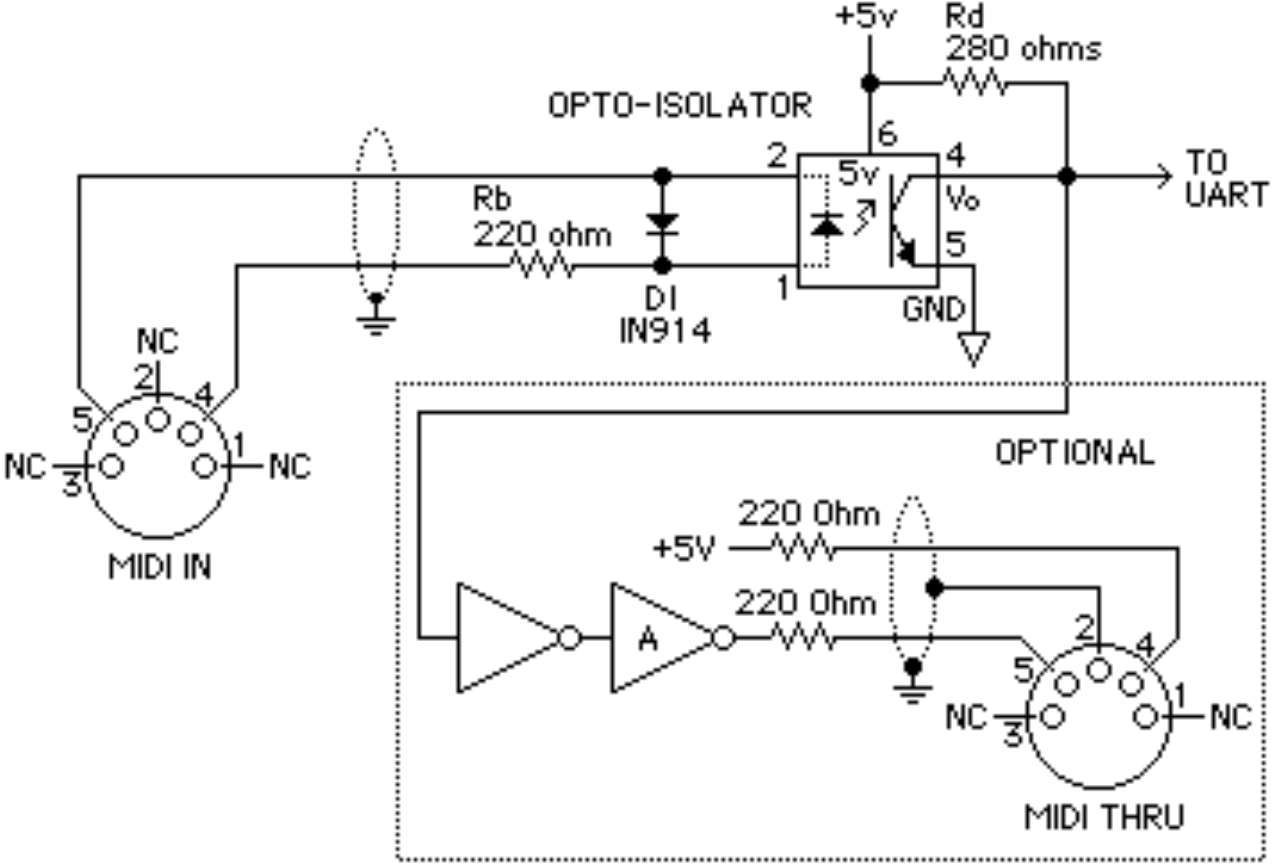
\includegraphics[width=0.7 \linewidth]{Images/midi-schematic.png}
    \caption{Schaltplan MIDI Eingang \cite[S. 2]{midi}}
    \label{fig:schaltplan-midi-inout}
\end{figure}

Rb dient zur Begrenzung des Stroms, D1 als Schutz vor Verpolung.
Als Optokoppler kommt ein 6n138 zum Einsatz. Rd ist dabei der Pullupwiderstand für das Ausgangssignal. Um das 31250 Baud-Signal trotz des intrinsisch langsamen Optokopplers ohne Verlust der Signalintegrität übertragen zu können, wird ein relativ geringer Pullupwiderstand von 280 Ohm verbaut.

\subsection{MIDI-Befehle}

Ein MIDI Befehl setzt sich aus 3 über eine serielle Verbindung übertragenen Bytes zusammen.
Im ersten Byte wird ein Statuscode übertragen, Bytes 2 und 3 enthalten Daten.
Statusbytes und Datenbytes lassen sich auch anhand des MSB unterscheiden. Bei Statusbytes ist das Most-Significant-Bit auf 1 gesetzt, bei Datenbytes auf 0.
In Tabelle (\ref{table:midi-commands}) sind einige der MIDI-Befehle aufgeschlüsselt.

\ctable[
  maxwidth=\linewidth,
  caption=Midi Befehlsübersicht \cite{wiki_midi},\cite{midi},
  botcap,
  pos=h,
  label=table:midi-commands
  ]{llllX}{}{%
  \FL
Status  & Byte1 & Byte 2    & Aktion        & Beschreibung\ML
0x9n    & 0xkk  & 0xvv      & Note On     & Beginnt das Spielen einer Note kk auf Kanal n mit Anschlagdynamik kk\NN
0x8n    & 0xkk  & 0xvv     & Note Off  &   Beendet das Spielen einer Note kk auf Kanal n mit \enquote{Release Velocity} kk\NN
0xBn 	& 0xcc 	& 0xvv 	     & Control Change &	Ändert den Zustand eines Controllers auf Kanal n (Instrumentenspzifisch) \NN
0xEn 	& 0xvv  & 0xww 	 & Pitch Bending & Ändert die Tonhöhe der gehaltenen Noten, ähnlich wie das Saitenziehen bei einer Gitarre \NN
0xF0…7 	& 0xx 	&           & System exclusive Message & Steuermeldungen, gerätespezifisch, Länge beliebig \NN
\LL}

Um die Datenübertragung zu beschleunigen, darf bei wiederholter Übertragung von Befehlen des gleichen Typs das Statusbyte ausgelassen werden.

Zusätzlich zu den hier genannten Befehlen nutzt MIDI \enquote{Active Sensing}.
Dabei wird im Abstand von 300 ms das Byte \texttt{0b00000001} übertragen.
Wenn diese Übertragung ausbleibt, kann ein lauschendes Gerät einen Ausfall des Übertragungskanals erkennen und das Spielen von Noten beenden.

\subsection{Hardwareentwurf des Midi-Interfaces}
\label{midi-hardwareentwurf}
Um die MIDI-Schnittstelle des Drumcomputers zu implementieren wurde eine Interfacemodul gebaut.
Dieses hat einen MIDI-Eingang sowie 12 Triggersignal-Ausgänge.
Zum Auswerten der Seriellen Midi Kommunikation nutzt das Midi-Modul ein Arduino UNO, das von hinten auf die Platine aufgesteckt wird.

Die Entscheidung für das Arduino fiel, da es bereits vorhanden war, den Anforderungen an die Pin-Anzahl und Systemleistung genügt und der verbaute ATmega328p Microcontroller mit einer Betriebsspannung von 5V läuft. Dadurch können eurorackkompatible Triggersignale ohne Pegelwandler ausgegeben werden.

Für die Eingangsschaltung wurde die Schaltung aus der MIDI-Spezifikation verwendet. Das über den Optokoppler isolierte Signal ist mit dem RX-Pin des Arduinos verbunden.

Zwölf Ausgänge des Mikrocontrollers wurden auf 3.5 mm Mono-Klinkenbuchsen geroutet, damit die Ausgehenden Triggersignale mit Patchkabeln zu die einzelnen Drummodule übertragen werden können.
Dabei besteht die Gefahr, dass mit dem Kabel eine der Betriebsspannungen berührt wird.
Zum Schutz des Microcontrollers wurden daher alle Ausgänge mit 220 Ohm Widerständen gegen Stromspitzen  geschützt.

Schaltpläne und Platinenlayouts finden sich in der beiliegenden Dokumentation.

\subsection{Implementierung der MIDI-Schnittstelle in C}
Die Implementierung des Programmcodes geschah in C, da die Programmierung des ATMega328p in C bereits bekannt war. Teile einer UART-Implementierung lagen aus anderen Lehrveranstaltungen bereits vor, was die Implementierung erleichtert hat.

Der Programmaufbau besteht aus zwei Hauptkomponenten: 
\begin{enumerate}
    \item Einem Zustandsautomaten, der in der Interruptroutine der seriellen Schnittstelle eingehende MIDI-Befehle entgegen nimmt.
    \item Einer periodisch ablaufenden Funktion, die die jeweiligen Ausgänge schaltet.
\end{enumerate}

Der Zustandsautomat der MIDI-Implementierung ist in Abbildung (\ref{fig:sm}) abgebildet.

\begin{figure}[h]
    \centering
    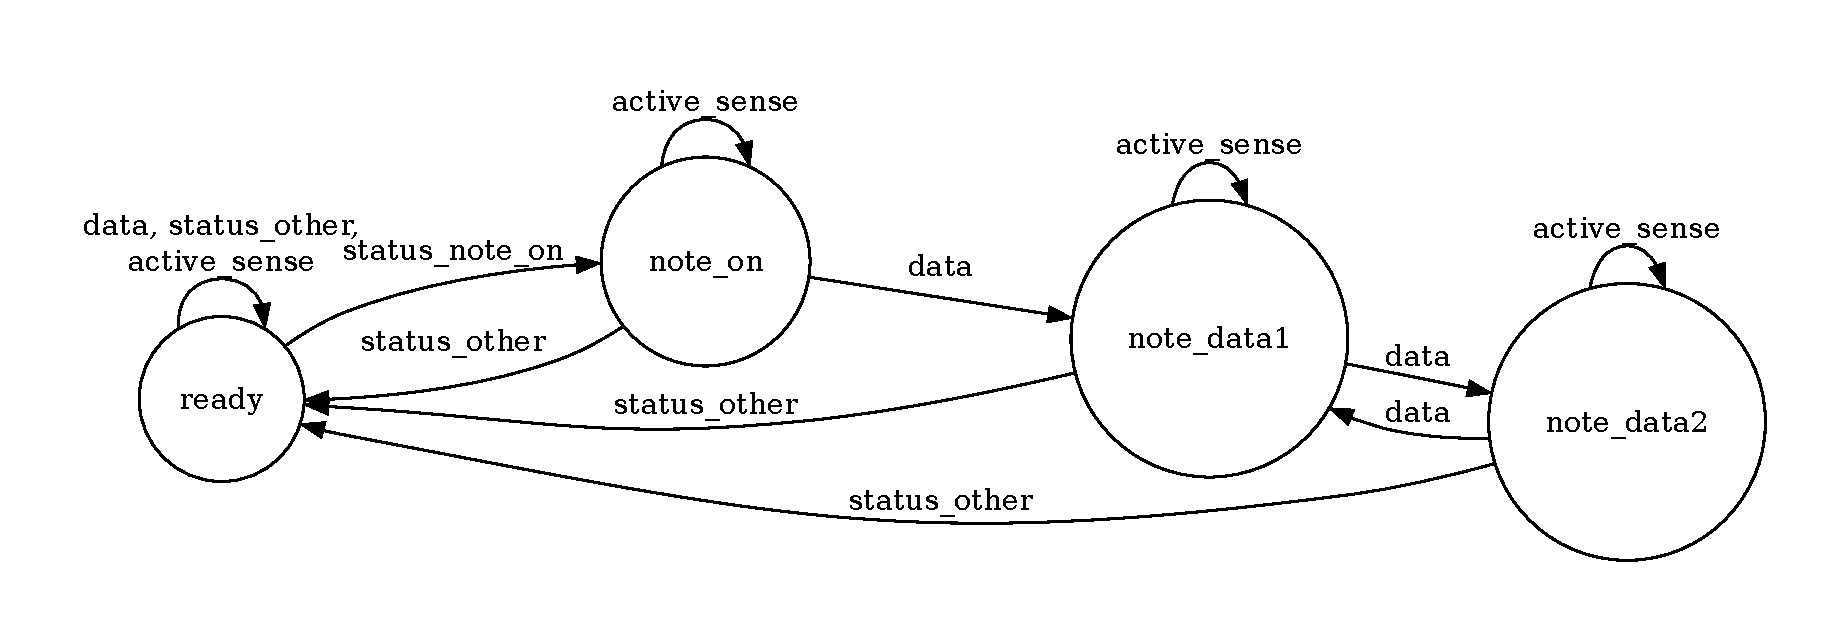
\includegraphics[width=0.9 \linewidth]{Images/sm.pdf}
    \caption{Zustandsautomat der Midi Implementierung}
    \label{fig:sm}
\end{figure}

Da nur Triggersignale generiert werden müssen, ist nur der Note-On Statuscode relevant. Die Ausgänge werden nach 1 ms wieder abgeschaltet, der Note-Off Befehl wird ignoriert.

Das Programm beginnt im Zustand \enquote{ready}.
Beim Empfang eines Note-On-Statuscodes geht der Automat in den Zustand \enquote{note\_on} über.

Beim Eingang des ersten Datenbytes wird in den Zustand \enquote{note\_data1} übergegangen, die über-tragenen Notenwerte werden in einer Variable gespeichert.

Nach der Übertragung des zweiten Datenbytes befindet sich der Automat im Zustand \enquote{note\_data2}.
Der zu schaltende Ausgang wird im Pufferspeicher markiert, die im zweiten Datenbyte übertragenen Velocitydaten sind für den Anwendungfall nicht relevant.

Bei Eingang eines weiteren Datenbytes wird in den Zustand \enquote{note\_data1} übergegangen. Dadurch wird die Übertragung mehrerer Note-On Befehle ohne wiederholung des Status-Bytes ermöglicht.

MIDI-Active-Sense Bytes, die regelmäßig übertragen werden um die Funktion des Datenkanals zu prüfen, werden ignoriert.

Bei Übertragung eines anderen Statusbefehls als Note-On wird in den Zustand \enquote{ready} gewechselt und auf Eingang eines Note-On Befehls gewartet.

In der Hauptschleife der \texttt{main}-Funktion werden die zu schaltenden Ausgänge aktiviert, anschließend wird für eine Millisekunde pausiert. So wird erreicht, dass die Triggersignale für genau eine Millisekunde aktiv sind. 
Dieser Schritt findet in einem Atomic-Block statt, sodass kein Interrupt das Schalten der Ausgänge unterbrechen kann.




